%% FEUP THESIS STYLE for LaTeX2e
%% how to use feupteses (English version)
%%
%% FEUP, JCL & JCF, 31 July 2012
%%
%% Read the documentation inline 
%% and at https://web.fe.up.pt/~jlopes/doku.php/doc/teach/feupteses
%%
%% PLEASE send improvements to jlopes at fe.up.pt and to jcf at fe.up.pt
%%

%%========================================
%% Commands: pdflatex tese
%%           bibtex tese
%%           makeindex tese (only if creating an index)
%%           pdflatex tese
%% Alternative:
%%          latexmk -pdf tese.tex
%%========================================

%% 2021-07-20: One-sided output by default
\documentclass[11pt,a4paper]{report}
%% For two-sided printing (for dead-tree output) comment previous line
%% and uncomment the next line
%% \documentclass[11pt,a4paper,twoside,openright]{report}

%% For iso-8859-1 (latin1), comment next line and uncomment the second line
\usepackage[utf8]{inputenc}
%\usepackage[latin1]{inputenc}

%% English version

%% MEIC options
\usepackage[meic]{feupteses}
%\usepackage[meic,juri]{feupteses}
%\usepackage[meic,final]{feupteses}
%\usepackage[meic,final,onpaper]{feupteses}

%% MEEC options
%\usepackage[meec]{feupteses}
%\usepackage[meec,juri]{feupteses}
%\usepackage[meec,final]{feupteses}

%% For other degrees
%\usepackage{feupteses} % you must define the degree bellow

%% Additional options for feupteses.sty: 
%% - onpaper: links are not shown (for paper versions)
%% - backrefs: include back references from bibliography to citation place

%% Uncomment to create an index (at the end of the document)
%\makeindex

%% Path to the figures directory
%% TIP: use folder ``figures'' to keep all your figures
\graphicspath{{figures/}}

%%----------------------------------------
%% TIP: if you want to define more macros, use an external file to keep them
%some macro definitions

% format
\newcommand{\class}[1]{{\normalfont\slshape #1\/}}

% entities
\newcommand{\Feup}{Faculdade de Engenharia da Universidade do Porto}

\newcommand{\svg}{\class{SVG}}
\newcommand{\scada}{\class{SCADA}}
\newcommand{\scadadms}{\class{SCADA/DMS}}

%%----------------------------------------

%%========================================
%% Start of document
%%========================================
\begin{document}

%%----------------------------------------
%% Information about the work
%%----------------------------------------
\title{Automatic Detection of Semantic Conflicts in Merge Commits via LLMs}
\author{Duarte Guedes Sardão}

%% Comment next line if not necessary for degree
%\degree{Programa Doutoral em Engenharia Informática}

%% Uncomment next line for date of submission
%\thesisdate{July 31, 2008}

%% Comment next line copyright text if not used
%\copyrightnotice{Name of the Author, 2008}

\supervisor{Supervisor}{José Campos}

%% Uncomment next line if necessary
%\supervisor{Second Supervisor}{Name of the Supervisor}

%% Uncomment committee stuff in the final version if used
%\committeetext{Approved by \ldots:}
%\committeemember{President}{Name of the President}
%\committeemember{Referee}{Name of the Referee}
%\committeemember{Referee}{Name of the Referee}

%% Uncomment signature line in the final on paper version if used
%\signature

%% Specify cover logo (in folder ``figures'')
\logo{uporto-feup.pdf}

%% Uncomment next line for additional text below the author's name (front page)
%\additionalfronttext{Preparação da Dissertação}

%%----------------------------------------
%% Preliminary materials
%%----------------------------------------

% remove unnecessary \include{} commands
\begin{Prolog}
  \chapter*{Resumo}
%\addcontentsline{toc}{chapter}{Resumo}

Em desenvolvimento de software colaborativo, trabalho paralelo, desenvolvido em diferentes ramos, tem de ser frequentemente integrado. Devido às diferenças do trabalho efetuado nos diferentes ramos, conflitos surgem frequentemente. Alguns conflitos são simples de detetar e rectificar, como conflitos de integração textuais, que surgem quando diferentes desenvolvedores editam a mesma linha em ramos diferentes: a maior parte de sistemas de controlo de versões consegue automaticamente detetar que a mesma linha foi alterada e impele o integrador a decidir numa solução: que alteração manter e que discartar.

Entre conflitos de integração, os semânticos emergem com um tipo particularmente difícil de resolver, porque não são detetados por sistemas de controlo de versões e, não tendo erros sintáticos, compilam com sucesso. Um exemplo de um conflito semântico pode ser visto numa classe Point, que contêm um método para calcular a distância para outro Point: num cenário em que um desenvolvedor num ramo A muda o cálculo de distância (de euclideana para manhattan, por exemplo), enquanto que outro chama o método dentro de uma função de movimento num ramo B, percebemos que depois de a integração nenhum erro é levantado, mas o comportamento está desviado dos ramos originais: especificamente, o movimento comportar-se-á de maneira diferente do que esperado no ramo B.

Procuramos explorar como o emergente ramo de Grandes Modelos de Linguagem podem fornecer um enorme avanço na nossa abilidade de testar o comportamento alterado, introduzido ou perdido devido a conflitos semânticos.
Especificamente, com base em trabalho anterior que identifica prováveis conflitos e gera outputs, numa linguagem de domínio específica, analisamos a abilidade de ChatGPT para gerar testes unitários apropriados that evidenciam a presença de conflitos semânticos, com prompting adequado.

\bigskip\noindent
\textbf{Palavras-chave:} LLM, Conflitos Semânticos, Geração de Testes

% ------------------------------------------------------------------------------

\chapter*{Abstract}
%\addcontentsline{toc}{chapter}{Abstract}

In collaborative software development, parallel work done by several different branches often has to be merged. Due to the differences of work done in the difference branches, often conflicts arise. Some conflicts are easy to detect and rectify, such as textual merge conflicts, where different developers have altered the same line in different branches: most version control systems can detect that the same line has been changed and urge the merger to decide on a solution, for example, by keeping one change and discarding the other.

Among merge conflicts, semantic merges arise as particularly difficult to resolve, as they avoid detection by version control systems and lacking syntactic errors, compile successfully. An example of a semantic conflict can be seen in a class such as Point, containing a method to calculate the distance to another Point: in a scenario where one developer in branch A changes the distance calculation (from euclidean to manhattan, for example), while another calls the distance method for a movement function in branch B, we find that upon a merge while no errors are raised, the code exhibits altered behaviour from the original branches: specifically, the movement will be different from what was developed in branch B.

We seek to explore how the emerging field of Large Language Models can provide a breakthrough in our ability to test for the altered, introduced and lost behaviours arising from semantic conflicts. Specifically, building upon previous work that identifies probable conflicts and generates outputs, on a domain-specific language, we analyse the ability of ChatGPT to generate appropriate unit tests that highlight the presence of semantic conflicts, given appropriate prompting.

\bigskip\noindent
\textbf{Keywords:} LLM, Semantic Conflicts, Test Generation
 % the abstract
  \chapter*{Acknowledgements}
%\addcontentsline{toc}{chapter}{Acknowledgements}

\todo{TBA}

\vspace{10mm}
\flushleft{Duarte Guedes Sardão}
  % the acknowledgments
  \cleardoublepage
\thispagestyle{plain}

\vspace*{8cm}

\begin{flushright}
   \textsl{``It takes a long time sometimes\\
   It can take a terrible long time before things sort themselves out.''} \\
\vspace*{1.5cm}
           Tove Jansson
\end{flushright}
    % initial quotation if desired
  \cleardoublepage
  \pdfbookmark[0]{Table of Contents}{contents}
  \tableofcontents
  \cleardoublepage
  \pdfbookmark[0]{List of Figures}{figures}
  \listoffigures
  \cleardoublepage
  \pdfbookmark[0]{List of Tables}{tables}
  \listoftables
  \chapter*{Abbreviations and Symbols}
%\addcontentsline{toc}{chapter}{Abbreviations}
\chaptermark{ABBREVIATIONS AND SYMBOLS}

\begin{flushleft}
\begin{tabular}{l p{0.8\linewidth}}
LLM      & Large Language Model\\
VCS     & Version Control System\\
DSL     & Domain Specific Language\\
\todo{are there others to be included here?} & \\
\end{tabular}
\end{flushleft}

  % the list of abbreviations used
\end{Prolog}

%%----------------------------------------
%% Body
%%----------------------------------------
\StartBody

%% TIP: use a separate file for each chapter
\chapter{Introduction} \label{chap:intro}

The purpose of this chapter is to introduce the motivation for the work, briefly describe the problem at hand and outline the work that will be developed, as well as the structure of the thesis.

\section{Motivation} \label{sec:motivation}

Collective software development requires the handling of merge conflicts, as conflicts between parallel work arise. Called merge conflicts, as they arise when this parallel work is merged, they vary in their difficulty of detection.
Common textual conflicts, where the same line is altered by multiple people, are automatically detected by version control systems, allowing amendments to be easily made. However not all conflicts are this easily detected and their introduction bring with it the addition of software bugs to the system. Semantic merge conflicts, in particular, are hard to detect, both by software and human review and remain a hard to solve situation.
The recent revolution in the field of Large Language Models (LLMs) may prove to add a valuable tool in tackling this.


\section{Problem} \label{sec:problem}

To manage the concurrent work of several developers in software projects, it is common to employ \emph{version control systems} (hereby referred as \emph{VCS}), which can be defined as "a system that manages the development of an evolving object. In other words, it is a system that records any changes made by the software developers." ~\citep{kn:vers_review}.

A significant task of version control is managing access to shared resources.
In the "classic scenario" a lock-modify-unlock paradigm was adopted, where a given file would be locked for modification while it is being modified, thus ensuring each resource can only be handled by one actor at a time. VCS's however, generally implement a copy-modify-merge mechanism: concurrent work can done on a resource, with joining the parallel work together handled by merges afterwards, with two "branches" of work merged into one. ~\citep{kn:vers_ott}

Merge conflicts arise when parallel work can't be clearly merged. Of this, several different types exist, as summarized by Tom Mens ~\citep{kn:tmens}:

Textual conflicts occur when the same textual elements of code are modified in both branches of a merge. For example, when the same line of code is modified by two people in their respective branches.

Syntactic conflicts arise from parallel changes that when merged don't generate textual conflicts, but the resulting merge creates code that is invalid given the languages rules. For example, programmer A renames a variable, while programmer B uses the variable somewhere (with the original name). There's no textual code, but the code won't compile due to the usage of an uninitialized variable.

Finally semantic conflicts occur when parallel changes don't trigger any conflict and are syntactically valid, but the resulting code doesn't behave as expected, or exhibits lost or new unexpected behaviour.

Most VCS's, such as Git, implement textual merge tools (ergo, they can only identify textual conflicts), however there are specialized tools that handle other types of merges: for example Turbomixer for syntactic merges.~\citep{kn:tmens} This focus on textual merging is generally fine as around 90\% of conflicts are textual ~\citep{kn:lcsd} and syntactic conflicts are easy to identify after merges, as errors will be clearly indicated and programs won't compile.
Semantic conflicts remain as both undetected by VCS's and hard to detect after merges. Thus, identifying methods to automatically identify and highlight semantic conflicts in merge commits has been a persistent problem and a source of study in this field. ~\citep{kn:nuno} ~\citep{kn:leuson} ~\citep{kn:leuson2}



\section{Goal and Approach} \label{sec:approach}

In previously developed work, a Domain-Specific Language was designed which describes the changes made in a three-way merge.~\citep{kn:nuno}. This DSL provides a summarized report of a three-way merge. We will feed the DSL reports into ChatGPT and induce it to generate unit tests based on them which should help assess the presence of a semantic conflict originating from the merge.






\section{Thesis Structure} \label{sec:struct}


Lorem ipsum 
\chapter{Related Work} \label{chap:sota}

\section{Introduction}

 The following chapters introduces the two main topics dealt with in this dissertation (merge conflicts and the usage of large language models for software verification and test generation). They explore related work and how we can build on it to develop our approach.

\section{Semantic Conflict Detection}

The study of merge techniques and conflicts has a long history, likely even predating the specific terminology itself. Thus there is a large corpus of work to explore

Several related works exist which seeks to develop methods that can more systemically identify adulterated behaviour arising from semantic conflicts.

\subsection{Automated Behaviour Change Detection}

By Da Silva et al, we find an attempt at identifying cases of semantic conflict by applying automated behaviour change detection~\citep{kn:leuson}. In summary, with a base commit B, a left L, right R and merge M, they observe that a generated unit test that passes in L but fails in B partially reveals the effect of the changes made in that branch. If the test then fails in M, it is likely the changes made in R interfere. To generate unit tests they used EvoSuite and Randoop~\citep{kn:randoop}
~\citep{kn:evosuite}.

In their analysis they found that the developed tool only detected interference in four out of 15 changes within merge scenarios that do actually suffer from interference, corresponding then to a recall of 0.267. While this is a very modest rate, it displayed no false positives (precision of 1) and thus could likely be integrated in a testing process to prune possible merge conflicts early, or further studied and refined.



\subsection{Unit Tests}

In identifying the presence of semantic conflicts in a merge conflict, developed solutions have focused on the automatic generation of unit tests. Building upon their previous work, Da Silva et al ~\citep{kn:leuson2} worked with this approach: by proposing SAM (SemAntic Merge), a tool that generates tests upon merges in Java. In summary, SAM initially does a simple textual merge to integrate the difference branches while identifying possible textual conflicts. After merging four program versions are built, to fully describe the merge scenario under test: Base, Left, Right, Merge. Source code transformations to improve testability are also part of the process, but optional. Finally, the test generation tools are fed objects serialized during the execution of existing test suites. After applying four test generations tools: Evosuite ~\citep{kn:evosuite}, Differential Evosuite, Randoop ~\citep{kn:randoop} and Randoop Clean, their own adapted version of Randoop, SAM executes the generated tests against the four versions of the program, identifies which tests failed, interpreting it with pre-defined interference criteria heuristics and from there reports conflicts, if detected ~\citep{kn:leuson2}.

With detections in 9 out of 28, it shows improvements over previous work: the authors specifically highlight the best performance when combining tests from only EvoSuite and Differential EvoSuite. In both cases, they highlight the ability of transformations (for example, making private fields public) to increase testability, showing moderate improvements in some tested scenarios: "We observe that the adoption of Testability Transformations help the tools
to detect behavior changes. In the same direction as for semantic conflict
detection, 20 additional changes are detected with testability executables,
when compared to the original executables (only 69 changes detected). From
the 19 false-negative cases observed in the experiment, we could detect
behavior changes in 11 of them. However, the reported behavior changes are
not caused by the changes involved in the semantic conflicts. So we can’t say
that the tools were close in these cases."  ~\citep{kn:leuson2}.


Nuno Castanho has proposed the tool UNSETTLE (aUtomatic uNit teSt gEneraTion for semanTic confLict dEtection) ~\citep{kn:nuno}. This tool is composed of two modules:

Changes-Matcher identifies the possible presence of semantic conflicts, by first computing the changes between different versions (base and variants) and then comparing it to a set of patterns describing common sources of conflicts as a base. From this it generates a DSL file, highlighting which methods and classes should be put under test to identify the conflict.

The second module is the test generator, a modified version of EvoSuite that takes the previously created artifact as an input to guide test generation.

Of particular interest to us is Changes-Matcher, as this is also the starting point for our work, with the usage of a LLM over EvoSuite for test generation instead.

\subsection{Regression Testing}

Ti Jao et al have proposed test oracles for program merges. Most significantly, not only do they support two and three way merges but also octopus merges. The developed tool, TOM, generates tests to identify unexpected and lost behaviour. \citep{kn:ji2022}

\section{Test Generation}

\subsection{Traditional Automatic Test Generation}

Traditional methods of automated test generation can be divided into random and search-based techniques. The former, being random, is simpler and faster, while the latter employs heuristics and search algorithms to fulfill some criteria, like maximizing code coverage.

Randoop is one such example of random test generation. Some of the disadvantages of this technique can be mitigated with the employment of feedback-direction. ~\citep{kn:randoop} Effectively, the search space of possible random tests is pruned, by guiding the test generator towards valid cases, avoiding expansion on invalid test cases~\citep{kn:randoop}.

Evosuite implements search-based automatic test generation for Java code, aiming for tests that achieve high coverage, while being as small as possible and providing assertions. To achieve this they implement both evolutionary search to evolve the suite with respect to a coverage criterion and mutation testing to generate assertions~\citep{kn:evosuite}.

EvosuiteR extends Evosuite, aiming to provide automated generation of regression tests. Thus it takes account two versions of the software and aside from coverage, it considers state distance ("how different is the state of
all objects in the test suite across the two versions") and control flow distance ("how
far are the two versions from diverging")~\citep{kn:evosuiter}.


Similar suites have been developed, for example, for Python ~\citep{kn:pynguin}.

\subsection{Test Generation with LLM's}

The recent explosion in complexity and popularity of LLM's has suscitated developer interest in their abilities with regards to accelerate and automate software engineering. Angela Fan et al identified that by 2023 3\% of pre-prints were related to Large Language Models and 11\% of those related to their use in software engineering.\cite{kn:angela} Particularly relevant is their ability to generate tests, with an expectation that they could achieve better coverage, correctness and readability than previous techniques of automated test generation.\cite{kn:junjiewang}
In comparison to traditional suites for automated test generation, such as EvoSuite, Palus, Randoop, and JTExpert, ChatGPT has shown, given right tuning of temperature settings, to evidentiate equivalent robustness\cite{kn:gptunitbra}.
From surveys done on the topic, we find Codex and GPT variants to be the most commonly used LLM's for this issue. \cite{kn:junjiewang}

While many studies suggest LLM's are competitive with traditional methods of software generation, we can also find evidence to the contrary. Specifically, testing across several LLM's, including Codex, StarCoder and GPT-3.5-Turbo, shows they fail in all regards compared to Evosuite, primarily due to the generation of non-compilable code, often due to "hallucination" of non-existent types and methods. \citep{kn:siddiq2023empirical}. Yutian Tang and others find Evosuite outperforms ChatGPT in code coverage. \citep{kn:tang2023chatgpt}. Given the novelty of the technology, it is unsurprising there is such variance in reported results and research, but it is worth investigating.

Despite variable conclusions regarding correctness and coverage, it seems generally agreed that ChatGPT is good at generating readable code. Yutian Tang et al highlight that despite minor style errors, primarily in identation, the generated code is clear and easy to understand. \citep{kn:tang2023chatgpt}. A survey of software developers has found ChatGPT to have comparable and even better readability than manually written tests. \citep{kn:chattester}


Given the LLM can produce unreliable results, the maximization of ChatGPT's abilities with regards to test generation has been explored: techniques such as prompting the LLM for a explanation of what the code is intending to do \cite{kn:nuances} and feeding error messages from codes that fail to compile or execute as intended back to the LLM for correction \cite{kn:chattester} have shown an amazing capacity for test generation, given the right prompting.

Regarding prompting, understanding how to best engineer prompts to achieve the desired output from the LLM is a particularly relevant issue. For example, in the generation of test inputs, research found “generate diverse test input” to be preferable over “generate test inputs that result in different outputs between PUT and reference versions”, as ChatGPT could not accurately identify the nuances required to correctly carry out the latter's instructions. \citep{kn:nuances}
With unit testing generation in particular, Zhiqiang Yuan et al, in developing the ChatTester tool, highlight the importance of combining a natural language descriptor with the appropriate code context. \citep{kn:chattester}
\begin{figure}[!h]
    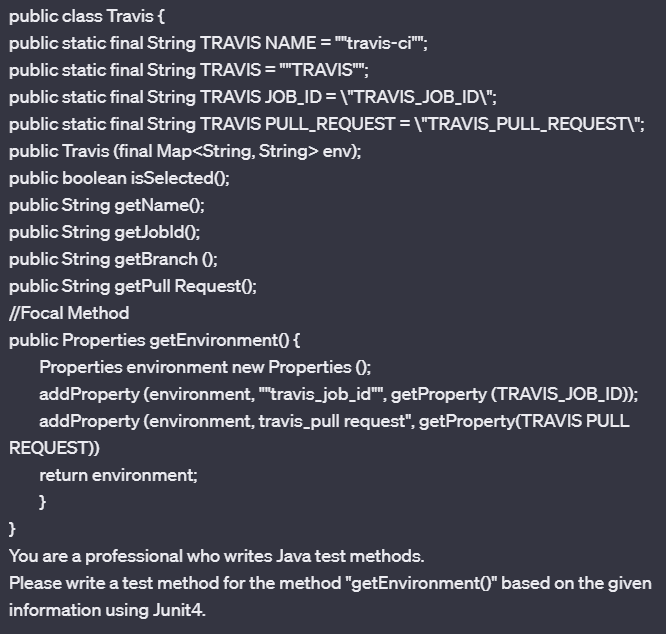
\includegraphics[width=0.86\textwidth]{figures/basicprompt.jpg}
    \caption{Basic Prompt in ChatTester}
    \label{fig:arch}
\end{figure}
\begin{figure}[!h]
    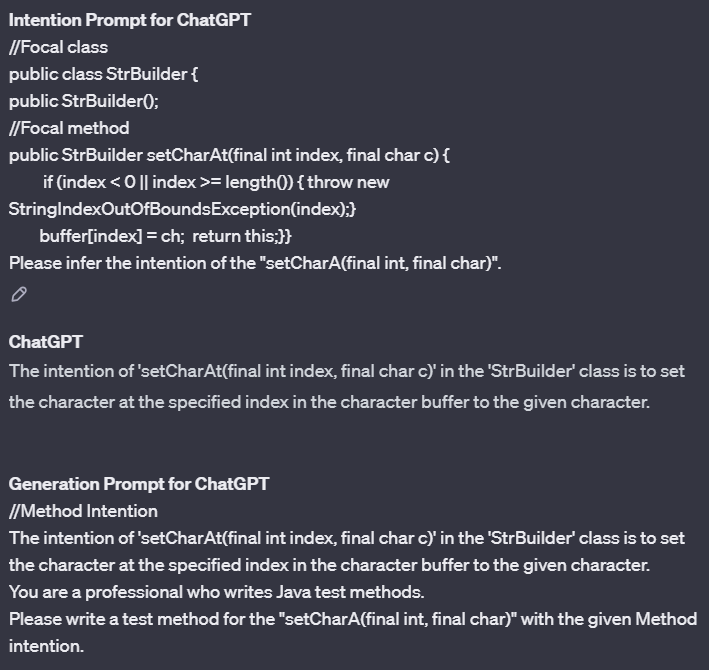
\includegraphics[width=0.86\textwidth]{figures/inferenceprompt.jpg}
    \caption{Inference Prompt in ChatTester}
    \label{fig:arch}
\end{figure}

The team behind ChatUniTest presents a two step prompting system, where instructions of what is to be done and how are first provided: "Please help me generate a JUnit test for a specific Java method using JUnit5 and Mockito3. I will provide the source code for the method, relevant method signatures and fields, required dependencies, Java class containing the method, expected behavior, and involved classes in the project. Create a test that imports necessary dependencies, compiles without errors, and achieves maximum branch and line coverage. No explanations needed.". This is followed by a prompt with the information proper for the creation of the test: "The focal method is ... in the class ... , and the class information is .... The brief information of involved class ... is ..." \citep{kn:chatunitest}


The training of LLM's in open source repositories gives cause to the fear that automatic test generation might be reliant on the model being trained in the code under test, or simply replicating existing testing suites. To assuage this, it was identified that even when generating tests for packages hosted in GitLab (which were not used to train the LLM under study, gpt3.5-turbo), they still maintained high coverage. In addition, it was found that 60.0\% of the tests had <= 40\% similarity to existing tests and 92.8\% had <= 50\%. Thus we can conclude the LLM is not simply copying tests from the training set without alteration.\citep{kn:max}.


\section{Conclusions}


The related work aids our own work in several ways: the work explored as regards unit test generation can provide show us a baseline functioning of the idea we're trying to implement. Particularly, we can use their statistics regarding percentage of conflicts found to assess whether our own solution is an improvement with regards to previous work.

Crucially important too is the work of Nuno Castanho and, as previously mentioned, the developed Changes-Matcher ~\citep{kn:nuno}.

The study of works on LLM test generation should also prove useful in the future, allowing us to get a better understanding of their functioning and capabilites, as well as providing ideas and prompt generation techniques which we may have to apply in the future.
\chapter{Preliminary and Future Work}\label{chap:chap3}

\section{Preliminary Work}

In the initial step of work, we superficially explored ChatGPT's ability to generate tests for an example conflict of Point, where a distance method is altered from euclidean to manhattan in one branch and in the other branch, a move method is changed from using the value 1 for x and y movement to using the result of the distance calculation.

We tested two frameworks, first just asking for a test, with prompts based on the testing indications given by the DSL for the case:

\begin{itemize}
  \item A Dependency Based semantic conflict was possibly introduced in a 3-way merge. Develop a test for the class Point, that covers the methods move() and distance(), without calling distance() directly.
Before the merge, the class under test was: [base Point]
After the merge, it was: [merged Point].
  \item A Dependency Based semantic conflict was possibly introduced in a 3-way merge. Develop a test for the class Point, that covers the methods move() and distance(), without calling distance() directly.
Before the merge, the class under test was: [base Point]
In the branch A it was changed to: [A Point]
In the branch B it was changed to: [B Point]
After the merge, it was: [merged Point].

\end{itemize}

For this, the LLM simply took one version and created tests taking it as correct behaviour. In the first case, for Base and in the second for Merge. This is not ideal, as the first does not allow us to distinguish if the behaviour changed due to merging, or just do to changes in the branches. The latter takes merge as correct behaviour and will thus always fail.

Other tests involved first asking for an explanation if there was a merge conflict there, before asking for a test

\begin{itemize}
  \item We have done a merge on a piece of code code.
Before the merge, the code was: [code]
In the branch A it was changed to: [code]
In the branch B it was changed to: [code]
After the merge it was: [code]
Do you believe there could be a merge conflict here? Where? Explain why.
  \item We have done a merge on a piece of code code.
Before the merge, the code was: [code]
In the branch A it was changed to: [code]
In the branch B it was changed to: [code]
After the merge it was: [code]
Do you believe there could be a merge conflict here? Where? Explain why. Pay attention to both additions and modifications.
  \item We have done a merge on a piece of code code.
Before the merge, the code was: [code]
In the branch A it was changed to: [code]
In the branch B it was changed to: [code]
After the merge it was: [code]
Do you believe there could be a *semantic* merge conflict here? Where? Explain why. Pay attention to both additions and modifications.

\end{itemize}

The first two prompts failed. Indeed for prompt ChatGPT only mentioned the changes in move, but even after prompting it to pay attention to distance, it failed to identify the conflict. For both, it seemed to not understand what was being referred to when speaking of conflict, describing all changes as a "conflict". Thus it would say, there is a conflict between whether to use euclidian and manhattan distance and there is a conflict on how the move function works.

The last prompt given, highlighting the *semantic* aspect of the merge conflict, yielded good results, with the conflict being perfectly described, as seen in figure \ref{fig:semconf}. After prompting for a test, it generates an appropriate one: it tests if the move function updates Point appropriately based on the euclidean distance. Thus it fails for base and branch B, where movement is still done with the value of 1, it passes for branch A as there move is based on distance; and it fails in merge, as now movement is being done with the distance calculation, but the calculation is now manhattan.

\begin{figure}
    \centering
    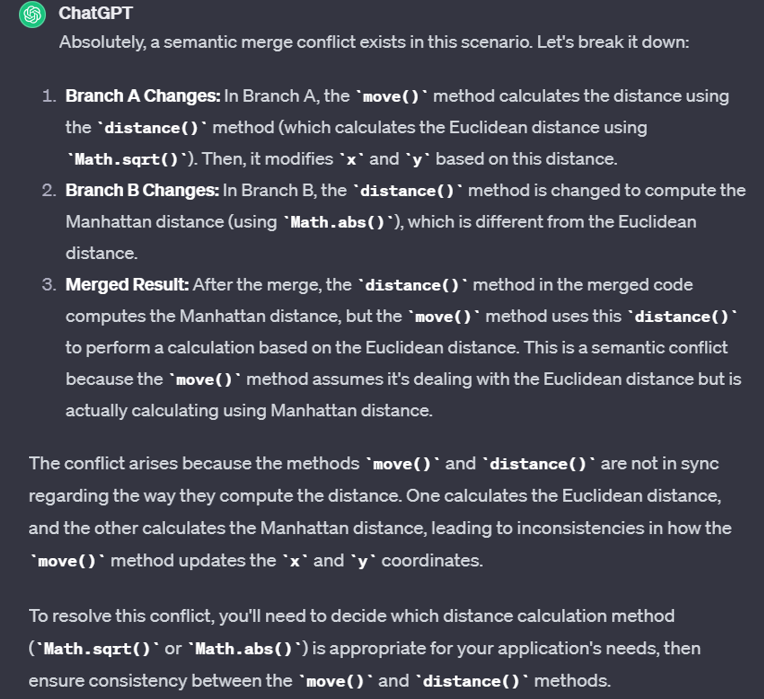
\includegraphics[width=0.75\linewidth]{figures/image.png}
    \caption{ChatGPT description of the semantic conflict}
    \label{fig:semconf}
\end{figure}

Prompting in real-world examples, or more complex fabricated examples, has produced far worse results. Common issues are confusion between textual and semantic merges, which can be mitigated by clear explanation of what a semantic merge is; hallucinations of features not present in the code or hallucinations of changes where changes were not made; lack of focus on the methods where conflict is evident, despite reiterations; loss of focus when prompt has to be split into several messages. When the tools do understand the semantic conflict, the best description they can give is to point out the changes made between branches followed by the suggestion that there may be a conflict there. No succesfull texts have been generated.
Experiments with other LLMs, such as Bing AI or Bard, yeld similar problems, suggesting an altered approach may have to be taken.



\section{Future Work}

\subsection{Development Plan and Tool Functioning}

Development of the solution will go through several stages. Firstly, the process which has already been in progress, is the initial evaluation of LLM's and prompt techniques. After acquiring the list of subjects to test and deciding on the LLM, we can systematize this to develop the prototype solution. From here we start developing a tool that can automatically generate a prompt, get a test from the LLM and then run it. This prototype tool can then be further augmented, by applying corrections for tests that may fail to compile. Figure \ref{fig:tool} details the expected functioning of the tool once completed. A final period of evaluation and observations will compare our results to previous work and reflect on possible further improvements.

\begin{figure}
    \centering
    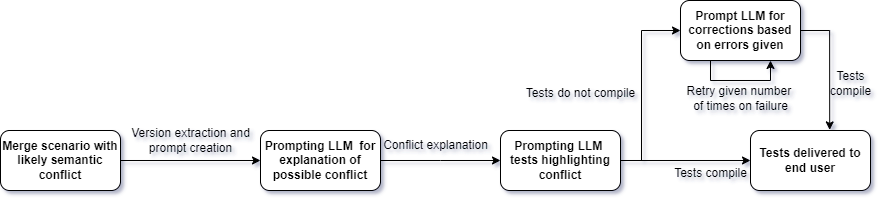
\includegraphics[width=1\linewidth]{figures/tool.png}
    \caption{Functioning pipeline of proposed tool}
    \label{fig:tool}
\end{figure}

\begin{figure}
    \centering
    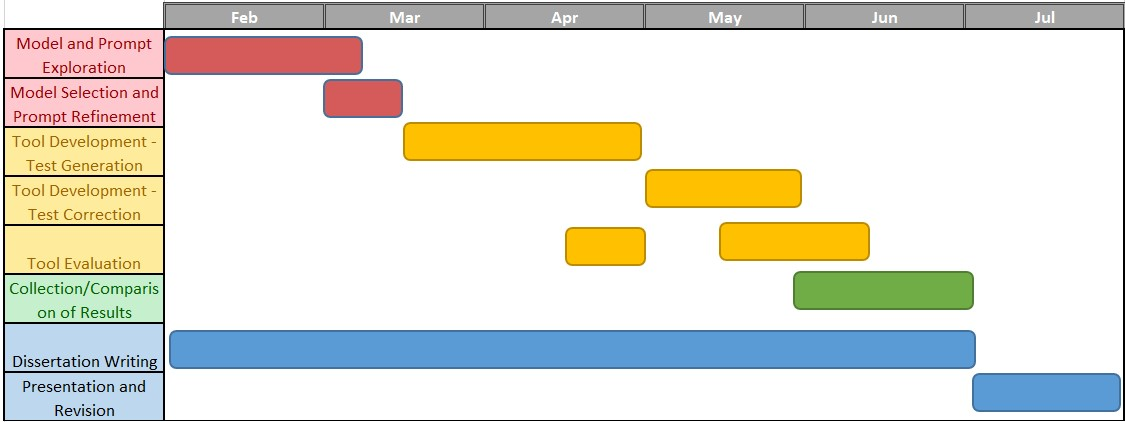
\includegraphics[width=1\linewidth]{figures/gantt.jpg}
    \caption{Gantt diagram of working plan}
    \label{fig:gantt}
\end{figure}

\subsection{Subjects}

To assess the validity of a developed solution, a collection of subjects to test must be collected. While several previous work has compiled collections of merge commits with semantic conflicts, the collection done by Nuno Castanho \cite{kn:nuno} is particularly useful, being publicly available, closely related to our own work, and also allowing us to draw direct comparisons. Most importantly, it aggregates merge instances from both Silva et al \cite{kn:leuson} and Sousa et al \cite{kn:safemerge}, thus being more extensive.

\subsection{LLM's}

While preliminary work sought to explore ChatGPT and Llama (both CodeLlama and Llama 2), hardware constraints meant we were unable to explore Llama. ChatGPT, being hosted online for free, did not suffer from such issues, but future problems may arise, most notably the possibility of the size limit for messages interfering in our work. Going forward we will further explore how to mitigate these and possible alternatives.
\chapter{Conclusion \& Future Work}\label{chap:chap4}

\section{Conclusion}

In our preparation for dissertation we explored and presented the problem of software merges, more specifically, the difficulty in establishing an automated method to detect, identify and highlight semantic conflicts that arise.

We explored related work that can provide avenues of study and structures to guide the development of our solution. Specifically, previous work on test generation to identify semantic conflicts, the state of the art of automated test generation and the usage of Large Language Models for test generation, with specific focus on the important of appropriate prompting as well as output correction.

Forward, we will apply this knowledge in developing a solution that can hopefully aid developer workflows by identifying and generating tests for semantic conflicts.

\section{Future Work}

\subsection{Development Plan and Tool Functioning}

Development of the solution will go through several stages. Firstly, the process which has already been in progress, is the initial evaluation of LLM's and prompt techniques. After acquiring the list of subjects to test and deciding on the LLM, we can systematize this to develop the prototype solution. From here we start developing a tool that can automatically generate a prompt, get a test from the LLM and then run it. This prototype tool can then be further augmented, by applying corrections for tests that may fail to compile. \Cref{fig:tool} details the expected functioning of the tool once completed. A final period of evaluation and observations will compare our results to previous work and reflect on possible further improvements.

\begin{figure}
    \centering
    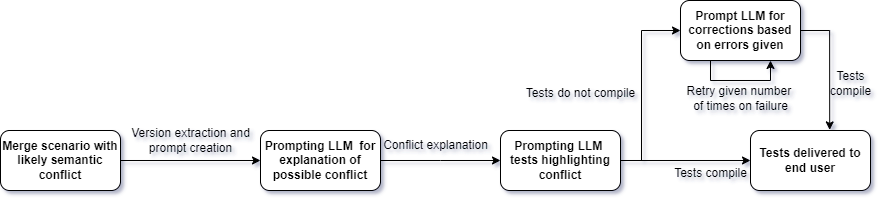
\includegraphics[width=1\linewidth]{figures/tool.png}
    \caption{Functioning pipeline of proposed tool}
    \label{fig:tool}
\end{figure}

\begin{figure}
    \centering
    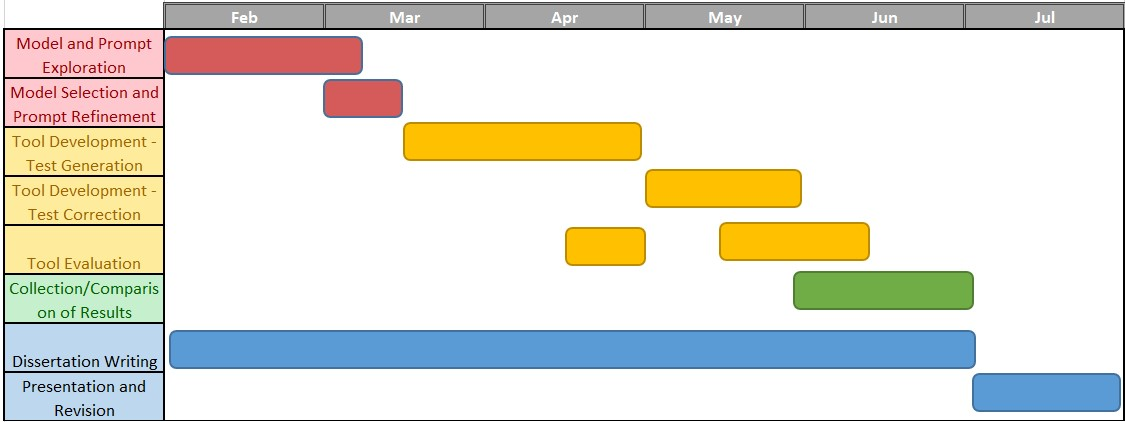
\includegraphics[width=1\linewidth]{figures/gantt.jpg}
    \caption{Gantt diagram of working plan}
    \label{fig:gantt}
\end{figure}

%\chapter{Conclusões e Trabalho Futuro} \label{chap:concl}

Proin sed justo eu sapien eleifend elementum. Pellentesque
habitant morbi tristique senectus et netus et malesuada fames ac
turpis egestas. Vivamus quam lacus, pharetra vel, aliquam vel,
volutpat sed, nisl. 

\section{Satisfação dos Objetivos}

Lorem ipsum dolor sit amet, consectetuer adipiscing elit. Etiam non
felis sed odio rutrum ultrices. Donec tempor dolor. Vivamus justo
neque, tempus id, ullamcorper in, pharetra non, tellus. Praesent eu
orci eu dolor congue gravida. Sed eu est. Donec pulvinar, lectus et
eleifend volutpat, diam sapien sollicitudin arcu, a sagittis libero
neque et dolor. Nam ligula. Cras tincidunt lectus quis nunc. Cras
tincidunt congue turpis. Nulla pede velit, sagittis a, faucibus vitae,
porttitor nec, ante. Nulla ut arcu. Cras eu augue at ipsum feugiat
hendrerit. Proin sed justo eu sapien eleifend elementum. Pellentesque
habitant morbi tristique senectus et netus et malesuada fames ac
turpis egestas. Vivamus quam lacus, pharetra vel, aliquam vel,
volutpat sed, nisl. 

Nullam erat est, vehicula id, tempor non, scelerisque at,
tellus. Pellentesque tincidunt, ante vehicula bibendum adipiscing,
lorem augue tempor felis, in dictum massa justo sed metus. Suspendisse
placerat, mi eget molestie sodales, tortor ante interdum dui, ac
sagittis est pede et lacus. Duis sapien. Nam ornare turpis et
magna. Etiam adipiscing adipiscing ipsum. Fusce sodales nisl a
arcu. Cras massa leo, vehicula facilisis, commodo a, molestie
faucibus, metus. Suspendisse potenti. Duis sagittis. Donec porta. Sed
urna. Maecenas eros. Vivamus erat ligula, pharetra sit amet, bibendum
et, fermentum sed, dolor. Nullam eleifend condimentum nibh. Integer
leo nibh, consequat eget, mollis et, sagittis ac, felis. Duis viverra
pede in pede. Phasellus molestie placerat leo. Praesent at tellus a
augue congue molestie. Proin sed justo eu sapien eleifend
elementum. Pellentesque habitant morbi tristique senectus et netus et
malesuada fames ac turpis egestas. 

\section{Trabalho Futuro}

Lorem ipsum dolor sit amet, consectetuer adipiscing elit. Aliquam
tempor tristique risus. Suspendisse potenti. Fusce id eros. In eu
enim. Praesent commodo leo. Nullam augue. Pellentesque tellus. Integer
pulvinar purus a dui convallis consectetuer. In adipiscing, orci vitae
lacinia semper, sapien elit posuere sem, ac euismod ipsum elit tempus
urna. Aliquam erat volutpat. Nullam suscipit augue sed
felis. Phasellus faucibus accumsan est. 

Aliquam felis justo, facilisis sit amet, bibendum ut, tempus ac,
dolor. Sed malesuada. Nunc non massa. In erat. Nulla
facilisi. Phasellus blandit, est in accumsan cursus, libero augue
elementum leo, vitae auctor mauris nisl ac tortor. Cras porttitor
ornare elit. Fusce at lorem. Sed lectus tortor, vestibulum id, varius
a, condimentum nec, lectus. Maecenas in nisi et magna pretium
aliquam. Pellentesque justo elit, feugiat nec, tincidunt a, dignissim
vel, ipsum. Sed nunc. Vestibulum ante ipsum primis in faucibus orci
luctus et ultrices posuere cubilia Curae; Aliquam tempus rhoncus
leo. Donec neque quam, cursus sit amet, ultricies varius, semper non,
pede. Donec porttitor. Sed aliquet feugiat elit.  

\vspace*{12mm}

Lorem ipsum dolor sit amet, consectetuer adipiscing elit. Phasellus
tellus pede, auctor ut, tincidunt a, consectetuer in, felis. Mauris
quis dolor et neque accumsan pellentesque. Donec dui magna,
scelerisque mattis, sagittis nec, porta quis, nulla. Vivamus quis
nisl. Etiam vitae nisl in diam vehicula viverra. Sed sollicitudin
scelerisque est. Nunc dapibus. Sed urna. Nulla gravida. Praesent
faucibus, risus ac lobortis dignissim, est tortor laoreet mauris,
dictum pellentesque nunc orci tincidunt tellus. Nullam pulvinar, leo
sed vestibulum euismod, ante ligula elementum pede, sit amet dapibus
lacus tortor ac nisl. Morbi libero. Integer sed dolor ac lectus
commodo iaculis. Donec ut odio.  
 

%%----------------------------------------
%% Final materials
%%----------------------------------------

%% Bibliography
%% Comment the next command if BibTeX file not used
%% bibliography is in ``myrefs.bib''
\PrintBib{myrefs}

%% 2021-07-20: change
%% comment next 2 commands if numbered appendices are not used
%\appendix
%\chapter{Extra stuff} \label{ap1:Lorem}

\section{Exploratory evaluation of ChatGPT's capabilities}

\subsection{Fabricated Examples}

In the initial step of work, we superficially explored ChatGPT's ability to generate tests for an example conflict of Point, where a distance method is altered from euclidean to manhattan in one branch and in the other branch, a move method is changed from using the value 1 for x and y movement to using the result of the distance calculation.

We tested two frameworks, first just asking for a test, with prompts based on the testing indications given by the DSL for the case:

\begin{itemize}
  \item A Dependency Based semantic conflict was possibly introduced in a 3-way merge. Develop a test for the class Point, that covers the methods move() and distance(), without calling distance() directly.
Before the merge, the class under test was: [base Point]
After the merge, it was: [merged Point].
  \item A Dependency Based semantic conflict was possibly introduced in a 3-way merge. Develop a test for the class Point, that covers the methods move() and distance(), without calling distance() directly.
Before the merge, the class under test was: [base Point]
In the branch A it was changed to: [A Point]
In the branch B it was changed to: [B Point]
After the merge, it was: [merged Point].

\end{itemize}

For this, the LLM simply took one version and created tests taking it as correct behaviour. In the first case, for Base and in the second for Merge. This is not ideal, as the first does not allow us to distinguish if the behaviour changed due to merging, or just do to changes in the branches. The latter takes merge as correct behaviour and will thus always fail.

Other tests involved first asking for an explanation if there was a merge conflict there, before asking for a test

\begin{itemize}
  \item We have done a merge on a piece of code.
Before the merge, the code was: [code]

In the branch A it was changed to: [code]

In the branch B it was changed to: [code]

After the merge it was: [code]

Do you believe there could be a merge conflict here? Where? Explain why.
  \item We have done a merge on a piece of code.
  
Before the merge, the code was: [code]

In the branch A it was changed to: [code]

In the branch B it was changed to: [code]

After the merge it was: [code]

Do you believe there could be a merge conflict here? Where? Explain why. Pay attention to both additions and modifications.
  \item We have done a merge on a piece of code code.
  
Before the merge, the code was: [code]

In the branch A it was changed to: [code]

In the branch B it was changed to: [code]

After the merge it was: [code]

Do you believe there could be a *semantic* merge conflict here? Where? Explain why. Pay attention to both additions and modifications.

\end{itemize}

The first two prompts failed. Indeed for prompt ChatGPT only mentioned the changes in move, but even after prompting it to pay attention to distance, it failed to identify the conflict. For both, it seemed to not understand what was being referred to when speaking of conflict, describing all changes as a "conflict". Thus it would say, there is a conflict between whether to use euclidian and manhattan distance and there is a conflict on how the move function works.

The last prompt given, highlighting the *semantic* aspect of the merge conflict, yielded good results, with the conflict being perfectly described, as seen in \Cref{fig:semconf}. After prompting for a test, it generates an appropriate one: it tests if the move function updates Point appropriately based on the euclidean distance. Thus it fails for base and branch B, where movement is still done with the value of 1, it passes for branch A as there move is based on distance; and it fails in merge, as now movement is being done with the distance calculation, but the calculation is now manhattan.

\begin{figure}
    \centering
    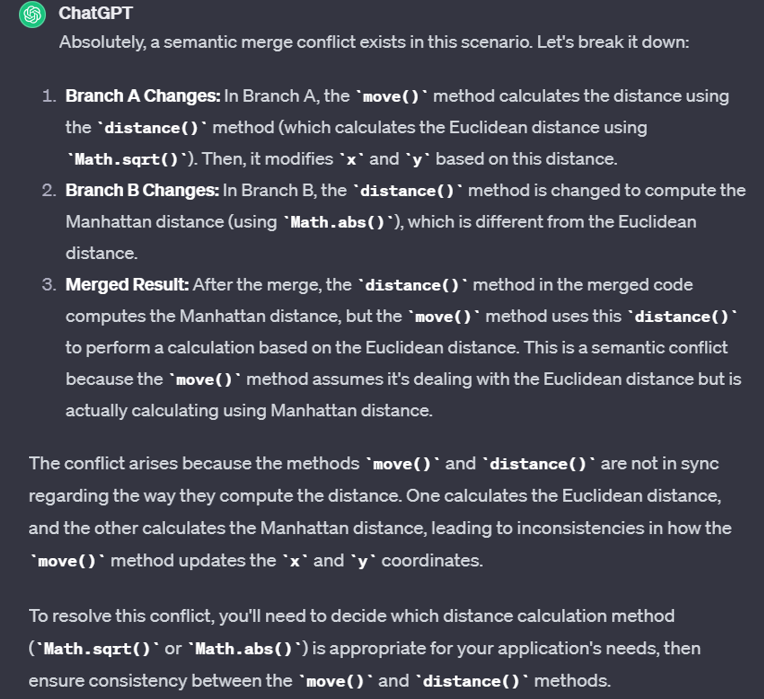
\includegraphics[width=0.75\linewidth]{figures/image.png}
    \caption{ChatGPT description of the semantic conflict}
    \label{fig:semconf}
\end{figure}

In simple fabricated scenarios, where simple conflicts were added to existing software solutions, ChatGPT showed ability to identify and describe the semantic conflict. Despite this, test generation remained complicated and few of the successful identification of semantic conflicts yielded working tests. The final prompt follows.

\begin{quote}
Generate a Junit unit test to identify this semantic conflict, knowing what you do now. The test must compile without errors and require no further alterations. It should require no further dependencies and import all classes correctly.
\end{quote}

While adapted to avoid common pitfalls, the tests generate still suffered from basic issues such as missing imports, which could be mitigated by prompting the LLM for correction automatically. More complex issues of implementation were present, such as calling the base function instead of dependent, wrong usage of construction and function returns, parameter types or unnecessary mocks. Further, when prompting for correction, the LLM often explains that the developer should correct this, thus further work needs to be done to ensure the tool does all the work itself.

\subsection{Real-World Merge Conflicts}

Prompting in real-world examples, or more complex fabricated examples, has produced far worse results. Several refinements were made to the prompts, most significantly: the usage of "git diff" to highlight the specific changes in branch A and branch B, the explanation of the conflict present and the specification of the target method where the conflict is evident. These modifications were largely unsuccessful and did not lead to identification of any significant amount conflicts.

We also had to reckon with size limits for messages. Thus, when necessary, we started with an explanatory prompt and then fed the information step by step. However, it remained crucial to remind the LLM of the goal in the last message.

\begin{quote}
We have done a merge on a piece of software and introduced a semantic conflict of types: "Update two different dependencies of a method or update one method and concurrently update one of its dependencies" and "Concurrent changes to the same method". I will now show the base commit, the diff in branch A, the diff in branch B, and the final merge version in 4 separate messages. At the end I want you to explain why and where the semantic conflict is present.
\end{quote}

Common issues are confusion between textual and semantic merges, which can be mitigated by clear explanation of what a semantic merge is; hallucinations of features not present in the code or hallucinations of changes where changes were not made; lack of focus on the methods where conflict is evident, despite reiterations; loss of focus when prompt has to be split into several messages. 
Rare close successes occured, particularly in cases where the conflict was asserted to be there in the prompt and could simply be described by explaining the changes made, such as parallel changes to collections initialization, as seen in \Cref{fig:cantfind}.

\begin{figure}
    \centering
    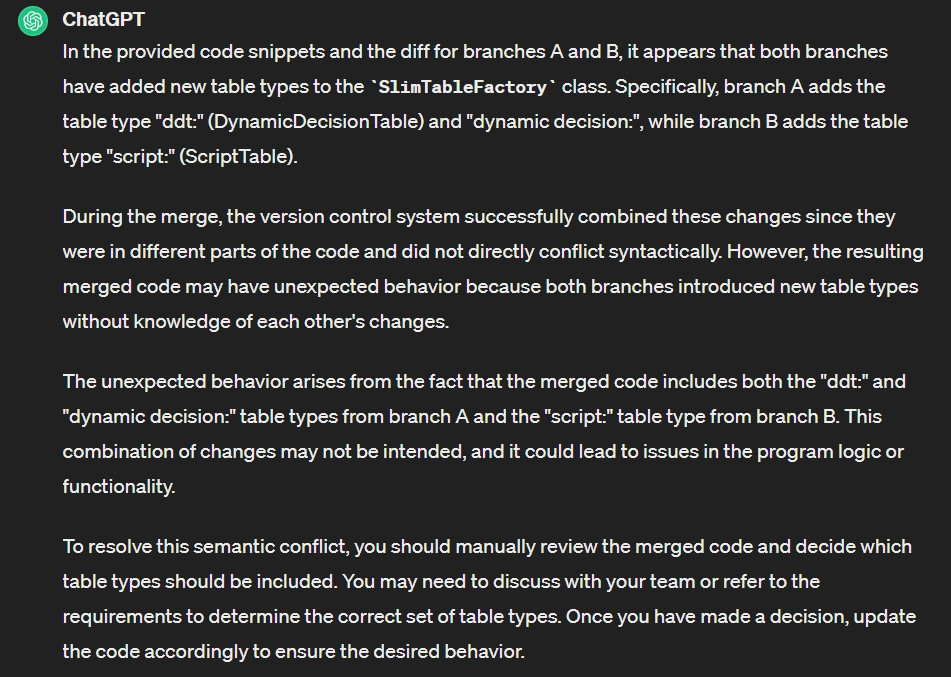
\includegraphics[width=1\linewidth]{figures/almostsemantic.jpg}
    \caption{ChatGPT describes the parallel changes as the origin of the conflict, but falls short of describing the emergent behaviour (in this case as simple as the different value returned by size())}
    \label{fig:cantfind}
\end{figure}

While we found that ChatGPT could not identify the semantic conflicts present in real software solutions, in some of \citet{kn:nuno}'s fabricated scenarios, these were correctly explained. Part of the difference between real-world examples and fabricated scenarios may come down to the information given. The fabricated scenarios were accompanied with a description of the specific semantic conflict present and the changes made perfectly reflected the description, with clear modifications and no extraneous changes. Thus it is possible collecting and offering that information with real-world scenarios may improve the ability of LLMs in this regard, but the higher "noise" of these scenarios may be too disruptive in this regard.

Another factor in consideration is the issue of dependencies, as so far testing had focused on just a unitary class. Given that semantic conflicts can involve interactions between classes and subclasses or other dependencies, it is relevant to provide further information. Initial tests just added one dependency, whether by calling a class methods or due to a inheritance relationship. An example, with the addition of an illustrative example of a semantic conflict follows.

\begin{quote}
We have done a merge on a piece of software and introduced a semantic conflict of type Parallel Changes in Method.

Semantic conflicts occur when concurrent and syntactic-correct changes in different regions of a source file or different files cause the software system to misbehave. For example, suppose there is a Java class `Point` with a method `distance()` that computes the Euclidean distance of a Point to the origin and Bob decides to modify `distance()` so it computes instead the Manhattan distance. At the same time, Alice, not aware of Bob's changes, creates a new method `move()` that uses `distance()` to calculate the Euclidean distance. Then, the changes of both developers are merged. As Bob and Alice did not modify the same lines of code, there is no textual conflict. There is neither a syntactic conflict as the merged code still compiles. However, the program now has an unexpected behaviour. The `move()` method introduced by Alice no longer moves a Point an Euclidean distance (as Alice was expecting) but rather moves a Manhattan distance

The affected declaration is copyWithDefaults().

A first message will detail the class before the merge, the diffs for both branches and the class after the merge. A second message will have a dependent class, whose methods indirectly call copyWithDefaults(). After I send these next two classes, identify and describe the semantic conflict.    
\end{quote}

A more complex evolution on this idea consisted of providing textual representations of UML graphs, such as plantUML call and structure graphs. These however proved to be complex in their own regard as they often induced the LLM to "forget" previous information and its goal, possibly due to their large size. A factor to consider, too, was that the information provided had to be limited in depth since, depending on the size of the software solution, a complete graph would be of extremely unwieldy size. Through some effort, we could get the LLM to recognize both the diagram and the class information, namely, by offering the diagram first.

\begin{quote}
We have done a merge on a piece of software. In this, we introduced a semantic conflict on the method dominates(State| State) of the class OpenTripPlanner. In a first message I will send a call diagram, in plantUML format. In a second message I will send the original class, the differences in the branches and the merged class.  At the end you must identify and explain the semantic conflict.
\end{quote}

However, it was particularly necessary to frequently refocus and concentrate the LLM. For example, after sending the diff and class information, reminding:

\begin{quote}
Explain why and where the semantic conflict is present, taking into account all the information provided in the last 2 messages. As mentioned before, focus on dominates(State| State). Make sure to mention information from the call diagram, if it is relevant to understanding the conflict.
\end{quote}

In the end, we were able to get the LLM to both recognize the merge information and the call diagram focused on the affected declaration and obtain a correct description of both the meaning of the diagram and the changes made in the merge. This however did not entail any improved description of the conflict, for all the cases tested.

Underscoring these experiments with real world test cases is an overlying issue: to properly identify a semantic conflict, we may have to analyze and take into account a large amount of data across several components of the software, while at the same time focusing on the specific components that were changed. While this is natural to a human, there is no clear way to select which information to feed and which to not in the LLM prompt: while a wider breadth of information may be necessary to identify the conflict, it is extremely likely to just induce further confusion and lead ChatGPT to focus on the wrong thing, or confuse different parts of code or even lose track of the task at hand as mentioned before.

\subsection{Test Generation without Conflict Understanding}

Given the difficulty of getting ChatGPT to provide accurate descriptions of the semantic conflicts, it was worth exploring whether the conflicts can be made evident just by generating tests targeting affected methods and classes. Several strategies were adopted: the prompting with the class after merge, the prompting with the class after merge and branch diffs and prompting with the class after merge and a structure graph. In most cases, where existing test suites where available, such information was also provided, with the prompt being reformulated to ask for its extension, rather than generation from scratch, as this shown to be important before~\cite{kn:githubcopilot}.

For 15 tests of 5 different projects, only 2 compiled, before and after prompting for corrections. One of these tested trivial additions to an array in both branches and the other identified a behaviour introduced in branch B that successfully carried over to merge, thus not a conflict. Positively, ChatGPT could understand the significance of this test working in branch B and merge but not A, as seen in \Cref{fig:testexplain}, suggesting it could understand the significance of a test failing for merge but not upper branches, which would indicate conflicts.

\begin{figure}
    \centering
    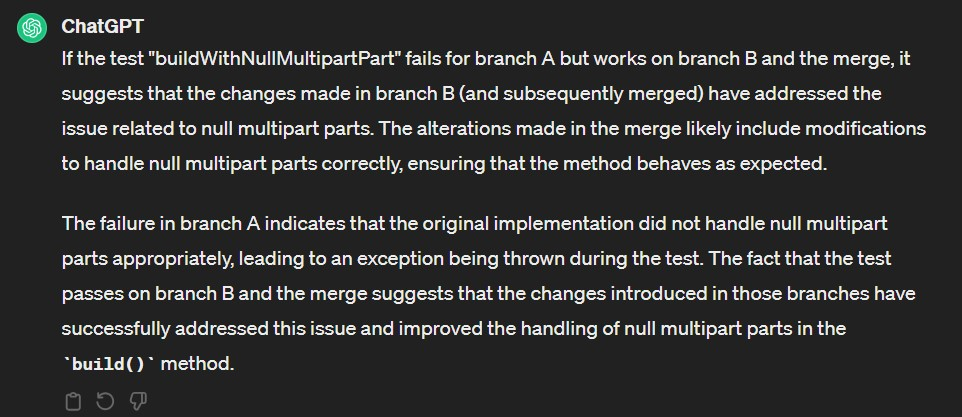
\includegraphics[width=1\linewidth]{figures/testexplain.jpg}
    \caption{ChatGPT explanation of meaning of failures and passes of test in different branches}
    \label{fig:testexplain}
\end{figure}

Common issues affecting test generation were:

\begin{itemize}
  \item Faulty importing/setup: Particularly relevant in the OKHttp case, the tool was patently unable to correctly call imports, just omitting them, even when expressly being given the package names and being told to import it.
  \item Invalid access: The LLM was generally unable to distinguish between private and public methods and frequently made attempts to invoke or access private methods and fields.
  \item Method/Field/Class Hallucination: ChatGPT frequently invoked non-existent methods, fields or even classes. In some classes this could also be related to matters of access, as it generated getter calls for private fields.
  \item Incomplete/Template Tests: Despite being prompted explicitly to generate complete tests that should compile, in several cases tests were generated with incomplete template helper methods and classes.
\end{itemize}

While feeding compilation error outputs could be a solution for these, in practice no test that failed to compile was fixed in this manner, as changes made did not fix or ignored the problems present. In some cases, while the logic of correction was sound logically, they were not helpful in the context of automatic test generation. For example, a "MockConverter" class was used in a test for the Retrofit project. Upon prompting for a fix, an import was added, which still naturally was non-functional. Upon prompting for another fix, ChatGPT provided a basic empty template for the MockConverter class. While a correctly implemented MockConverter class would fix the issue and allow the test to compile, the solution here would have been to drop the usage of the MockConverter class in the first place

Experiments were made to employ the usage of vector indexing to boost the capabilities of understanding code. The theory was that, by indexing the entire repository of code, we could proceed with prompting without having to decide which specific blocks of code should be required information in the prompt and that, during generation, the LLM could correctly identify the chain of dependencies, and which methods and parameters should be employed to properly test our desired methods. In this process we employed llama\_index, but the results fell short: due to an observed worse ability to generating code, focus was placed on the explanation of what should be done, with the prompting: "We want to create an extensive testing suite for the method [method] of the class [class]. How should we approach this? Which calls should we make, which parameters should we try and which results should be expected?"
Results were generic, many times not even referring to aspects of the code itself and still prone issues of hallucination, specifically the making of references to non-existent methods.

\section{Comparison of Developed Prompts with State of the Art}

To evaluated our progressively developed prompt with existing state of the art, we selected 5 prompts from comparison, henceforth referred as 1 \cite{kn:chattester}, 2 \cite{kn:siddiq2023empirical}, 3 \cite{kn:gptunitbra}, and 4 \cite{kn:chatunitest}. Our prompt, in turn, was 2-step prompt as follows:

\begin{quote}
The following class was altered in a merge, specifically the METHOD method. Analyse it and what it does, with focus on the method and its usage: CLASS INFO
\end{quote}

\begin{quote}
You are a Java developer. Due to changes in the METHOD method, you've been asked to write a complete test suite to identify possible errors introduced due to the changes. Write a junit test suite for the method. All classes must be correctly imported. The tests must compile without errors. The tests must be complete and require no modification and addition. No explanation needed.
\end{quote}

As subjects, we selected the basic fabricated Point class example, Antlr4, whose testing simply requires the length of a returned list and OkHttp, a more complex example requiring mocks and reflection for testing.
For each prompt, we generated 3 times and selected the best result for comparison.

For Point, we made the following observations:

Our prompt generated a suite with 3 tests, one of which had an incorrect assertion (A Point with coordinates -3,-4 was expected to move to 4,5 when it should move to 4,3). Despite this one wrong test, the correct ones successfully identified the conflict, as they tested manhattan distance movement. For an earlier branch, with euclidian distance movement, they would fail, showing the conflict.

Prompt 1 called the distance() method to identify where the Point should be and set assertions accordingly. While this tested the move method, it could not identify the conflict, as the assertions were dependent on the behaviour of distance(), as it changed so did they.

Prompt's 2,3,4 all made the same mistake: Starting from a point 3,4, they expected it to move to 7,8. As distance is 7, it should actually move to 10,11. Notably, Prompt 3 and 4 generated tests for distance and correctly identified it as 7.

For Antlr4, our prompt ran into errors: it could not correctly initialize the class, as the CodeGenerator object called by the constructor was incorrectly created. It also severely undercounted the number of keywords, leading to an incorrect assertion.
Prompt 1 showed improvement over ours, as it understood a null could be used in place of CodeGenerator, as it would not be used for our purposes. Despite this, it failed in the logic of the test, calling badWords unnecessarily: this is a private method that is already called by the getBadWords method we are testing. This same error was present in Prompt 2.
Prompt 3 generated nonsensical tests, just checking if the result of methods called was false. While it tested non-existent methods, it did not tested getBadWords as we desired.
Prompt 4 also called addBadWords despite not needing it, but as it was instructed to use Mockito, it avoided the error of calling a private method by using reflection. The rest of the test logic and the assertion was correct.


OkHttp should be the hardest to test, as the method under test and the method which calls it are private. The value returned (which we seek to test) is never publicly available.
Thus all prompts try and fail to call the private method. The exception is Prompt 3 which, by it's nature of generating for all methods rather than being told to generate for a specific one, avoids private methods. Surprisingly, Prompt 4 which had shown ability to use reflection in the previous subject, failed to produce a satisfactory result. Also of note is Prompt 2, which calls for 10 tests to be generated: in this case, to reach this 'quota', each parameter of the copied client was tested in a entirely different test, rather than just in a different assertion.
Despite failing, due to previously mentioned issue with access, Prompt 1 notably produced the best assertions, as it tested both functionalities of the method: the correct copying of defined parameters, and the returning of defaults for parameters that were not set.


%% Index
%% Uncomment next command if index is required
%% don't forget to run ``makeindex thesis'' command
%\PrintIndex

\end{document}
